% workflow.tex -- v3 Figure 3 (slug workflow), Step 4.2 (2026-09-03).
% The design-conditional elicitation workflow: the six steps of Box 1 with the
% three design settings named in the input box. Identity-free standalone source;
% compile with pdflatex to workflow.pdf (natural size, at most 4.8 x 5.0 in;
% included in the manuscript with no width argument). No implementation
% vocabulary; the stage names equal the recipe steps of Box 1.
\documentclass[tikz,border=2pt]{standalone}
\usepackage{amsmath,amssymb}
\usepackage[scaled=0.92]{helvet}
\renewcommand{\familydefault}{\sfdefault}
\usetikzlibrary{arrows.meta,positioning,shapes.geometric,fit,backgrounds,calc}
\begin{document}
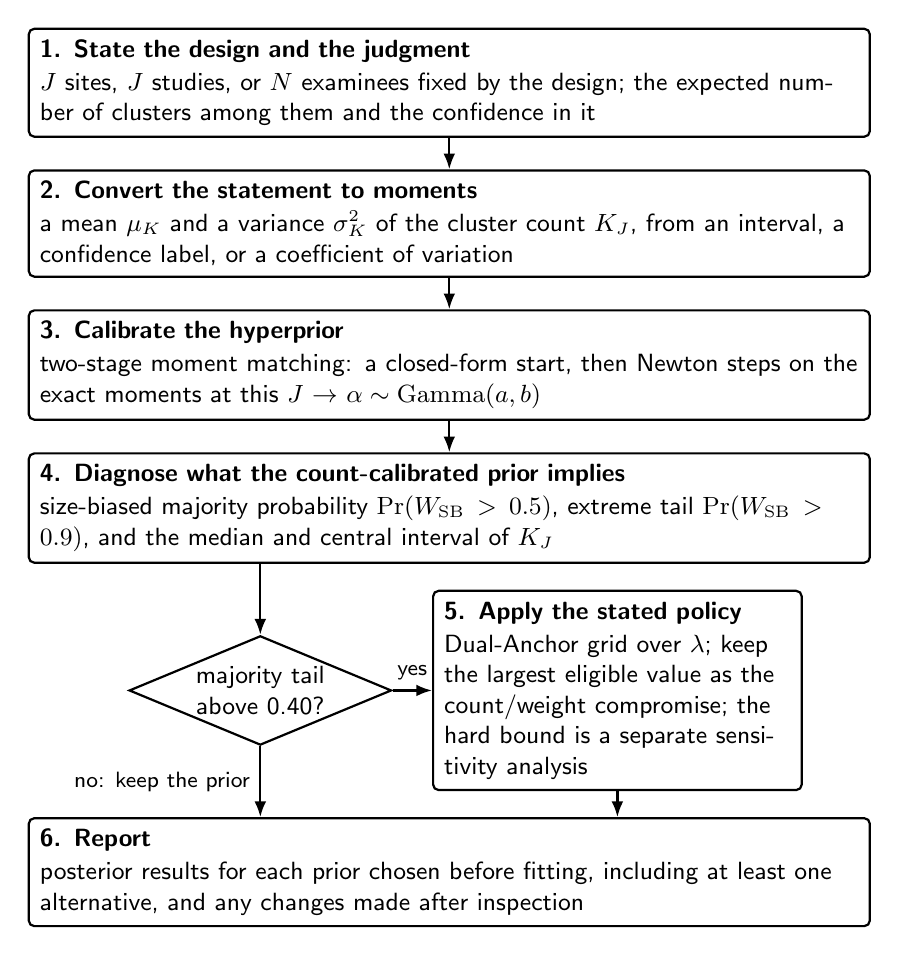
\begin{tikzpicture}[
  font=\small,
  >={Latex[length=2mm]},
  stepbox/.style={rectangle, rounded corners=2pt, draw=black, thick, align=left,
               text width=10.4cm, inner sep=4pt, fill=white},
  side/.style={rectangle, rounded corners=2pt, draw=black, thick, align=left,
               text width=4.4cm, inner sep=4pt, fill=white},
  decision/.style={diamond, draw=black, thick, aspect=2.4, align=center, inner sep=1pt, fill=white},
  group/.style={rectangle, rounded corners=4pt, draw=black!50, dashed, fill=black!4, inner sep=6pt},
  lab/.style={font=\footnotesize},
  num/.style={font=\bfseries}
]
\node[stepbox] (s1) {\textbf{1. State the design and the judgment}\\[1pt]
  $J$ sites, $J$ studies, or $N$ examinees fixed by the design; the expected number of clusters among them and the confidence in it};
\node[stepbox, below=4mm of s1] (s2) {\textbf{2. Convert the statement to moments}\\[1pt]
  a mean $\mu_K$ and a variance $\sigma_K^2$ of the cluster count $K_J$, from an interval, a confidence label, or a coefficient of variation};
\node[stepbox, below=4mm of s2] (s3) {\textbf{3. Calibrate the hyperprior}\\[1pt]
  two-stage moment matching: a closed-form start, then Newton steps on the exact moments at this $J$ $\rightarrow$ $\alpha \sim \mathrm{Gamma}(a, b)$};
\node[stepbox, below=4mm of s3] (s4) {\textbf{4. Diagnose what the count-calibrated prior implies}\\[1pt]
  size-biased majority probability $\Pr(W_{\mathrm{SB}} > 0.5)$, extreme tail $\Pr(W_{\mathrm{SB}} > 0.9)$, and the median and central interval of $K_J$};
\node[decision, below=9mm of s4, xshift=-2.4cm] (d) {majority tail\\above 0.40?};
\node[side, right=5mm of d] (s5) {\textbf{5. Apply the stated policy}\\[1pt]
  Dual-Anchor grid over $\lambda$; keep the largest eligible value as the count/weight compromise; the hard bound is a separate sensitivity analysis};
\node[stepbox, below=9mm of d, xshift=2.4cm] (s6) {\textbf{6. Report}\\[1pt]
  posterior results for each prior chosen before fitting, including at least one alternative, and any changes made after inspection};
\draw[->, thick] (s1) -- (s2);
\draw[->, thick] (s2) -- (s3);
\draw[->, thick] (s3) -- (s4);
\draw[->, thick] (s4.south -| d.north) -- (d.north);
\draw[->, thick] (d.south) -- node[lab, left] {no: keep the prior} (d.south |- s6.north);
\draw[->, thick] (d) -- node[lab, above] {yes} (s5);
\draw[->, thick] (s5.south) -- (s5.south |- s6.north);
\end{tikzpicture}
\end{document}
